\documentclass[tikz,border=8pt]{standalone}
\usepackage{amsmath,amssymb}
\usetikzlibrary{arrows.meta,calc,decorations.pathreplacing}

\begin{document}
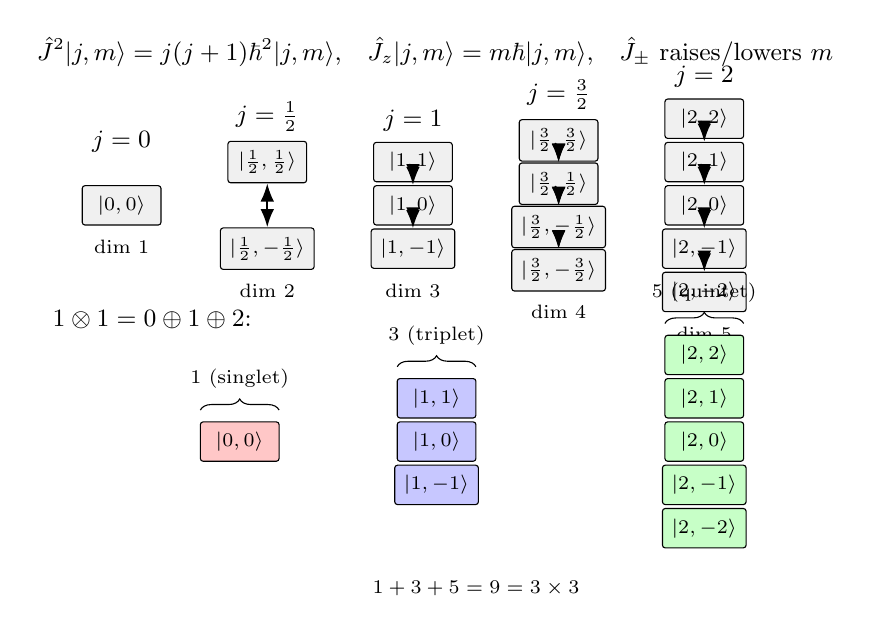
\begin{tikzpicture}[>=Latex,
  ket/.style={draw, fill=gray!12, minimum width=1.0cm, minimum height=0.5cm, font=\scriptsize, rounded corners=1pt}]

  \def\colsep{1.85}
  \def\rowstep{0.55}

  % j=0
  \begin{scope}[xshift=0cm]
    \node[ket] (a00) at (0, 0) {$|0,0\rangle$};
    \node[font=\small, anchor=south] at (0, 0.55) {$j=0$};
    \node[font=\scriptsize, anchor=north] at (0, -0.32) {dim 1};
  \end{scope}

  % j=1/2
  \begin{scope}[xshift=\colsep cm]
    \node[ket] (h1) at (0,  \rowstep) {$|\tfrac12,\tfrac12\rangle$};
    \node[ket] (h2) at (0, -\rowstep) {$|\tfrac12,-\tfrac12\rangle$};
    \draw[<->, thick] (h1) -- (h2);
    \node[font=\small, anchor=south] at (0, \rowstep+0.27) {$j=\tfrac12$};
    \node[font=\scriptsize, anchor=north] at (0, -\rowstep-0.32) {dim 2};
  \end{scope}

  % j=1
  \begin{scope}[xshift=2*\colsep cm]
    \node[ket] (o1) at (0,  \rowstep) {$|1,1\rangle$};
    \node[ket] (o2) at (0,  0)         {$|1,0\rangle$};
    \node[ket] (o3) at (0, -\rowstep) {$|1,-1\rangle$};
    \draw[<->, thick] (o1) -- (o2);
    \draw[<->, thick] (o2) -- (o3);
    \node[font=\small, anchor=south] at (0, \rowstep+0.27) {$j=1$};
    \node[font=\scriptsize, anchor=north] at (0, -\rowstep-0.32) {dim 3};
  \end{scope}

  % j=3/2
  \begin{scope}[xshift=3*\colsep cm]
    \node[ket] (t1) at (0,  1.5*\rowstep) {$|\tfrac32,\tfrac32\rangle$};
    \node[ket] (t2) at (0,  0.5*\rowstep) {$|\tfrac32,\tfrac12\rangle$};
    \node[ket] (t3) at (0, -0.5*\rowstep) {$|\tfrac32,-\tfrac12\rangle$};
    \node[ket] (t4) at (0, -1.5*\rowstep) {$|\tfrac32,-\tfrac32\rangle$};
    \draw[<->, thick] (t1) -- (t2);
    \draw[<->, thick] (t2) -- (t3);
    \draw[<->, thick] (t3) -- (t4);
    \node[font=\small, anchor=south] at (0, 1.5*\rowstep+0.27) {$j=\tfrac32$};
    \node[font=\scriptsize, anchor=north] at (0, -1.5*\rowstep-0.32) {dim 4};
  \end{scope}

  % j=2
  \begin{scope}[xshift=4*\colsep cm]
    \node[ket] (f1) at (0,  2*\rowstep) {$|2,2\rangle$};
    \node[ket] (f2) at (0,    \rowstep) {$|2,1\rangle$};
    \node[ket] (f3) at (0,  0)           {$|2,0\rangle$};
    \node[ket] (f4) at (0,   -\rowstep) {$|2,-1\rangle$};
    \node[ket] (f5) at (0, -2*\rowstep) {$|2,-2\rangle$};
    \draw[<->, thick] (f1) -- (f2);
    \draw[<->, thick] (f2) -- (f3);
    \draw[<->, thick] (f3) -- (f4);
    \draw[<->, thick] (f4) -- (f5);
    \node[font=\small, anchor=south] at (0, 2*\rowstep+0.27) {$j=2$};
    \node[font=\scriptsize, anchor=north] at (0, -2*\rowstep-0.32) {dim 5};
  \end{scope}

  % top label
  \node[font=\small, anchor=west] at (-1.2, 1.95) {$\hat J^2|j,m\rangle=j(j+1)\hbar^2|j,m\rangle$,\quad $\hat J_z|j,m\rangle=m\hbar|j,m\rangle$,\quad $\hat J_\pm$ raises/lowers $m$};

  % Bottom: 1 ⊗ 1 decomposition
  \begin{scope}[yshift=-3.0cm, xshift=0cm]
    \node[font=\small, anchor=west] at (-1.0, 1.55) {$1\otimes 1 = 0\oplus 1\oplus 2$:};

    % singlet
    \node[ket, fill=red!22] (s0) at (1.5, 0) {$|0,0\rangle$};
    \draw[decorate, decoration={brace, amplitude=4pt}] (1.0, 0.4) -- (2.0, 0.4);
    \node[font=\scriptsize, anchor=south] at (1.5, 0.55) {$1$ (singlet)};

    % triplet
    \begin{scope}[xshift=4cm]
      \node[ket, fill=blue!22] (tt1) at (0,  \rowstep) {$|1,1\rangle$};
      \node[ket, fill=blue!22] (tt2) at (0,  0)         {$|1,0\rangle$};
      \node[ket, fill=blue!22] (tt3) at (0, -\rowstep) {$|1,-1\rangle$};
      \draw[decorate, decoration={brace, amplitude=4pt}] (-0.5, \rowstep+0.4) -- (0.5, \rowstep+0.4);
      \node[font=\scriptsize, anchor=south] at (0, \rowstep+0.55) {$3$ (triplet)};
    \end{scope}

    % quintet
    \begin{scope}[xshift=7.4cm]
      \node[ket, fill=green!22] (q1) at (0,  2*\rowstep) {$|2,2\rangle$};
      \node[ket, fill=green!22] (q2) at (0,    \rowstep) {$|2,1\rangle$};
      \node[ket, fill=green!22] (q3) at (0,  0)           {$|2,0\rangle$};
      \node[ket, fill=green!22] (q4) at (0,   -\rowstep) {$|2,-1\rangle$};
      \node[ket, fill=green!22] (q5) at (0, -2*\rowstep) {$|2,-2\rangle$};
      \draw[decorate, decoration={brace, amplitude=4pt}] (-0.5, 2*\rowstep+0.4) -- (0.5, 2*\rowstep+0.4);
      \node[font=\scriptsize, anchor=south] at (0, 2*\rowstep+0.55) {$5$ (quintet)};
    \end{scope}

    \node[font=\scriptsize, anchor=north] at (4.5, -2*\rowstep-0.55) {$1+3+5=9=3\times 3$};
  \end{scope}
\end{tikzpicture}
\end{document}
